\documentclass{llncs}

\usepackage{url}
\usepackage{graphicx}
\usepackage{listings}
\usepackage{verbatim}
\usepackage[lined,linesnumbered,algochapter]{algorithm2e}
\usepackage{tikz}
\usetikzlibrary{arrows,automata}
\usepackage{xspace}

\usepackage{ngerman}
\usepackage[ngerman, english]{babel}
\usepackage[utf8]{inputenc}
\usepackage{bibgerm,cite}       % Deutsche Bezeichnungen, Automatisches Zusammenfassen von Literaturstellen
\usepackage[ngerman]{varioref}  % Querverweise

\setcounter{secnumdepth}{2}
\setcounter{tocdepth}{3}

% define custom macros for specific formats or names
\newcommand{\uml}[1]{\texttt{#1}}
\newcommand{\cd}{\textsf{Class Diagram}}

\begin{document}
\pagestyle{plain}
\pagenumbering{roman}

\title{Wissenschaftliches Arbeiten (188.925 - WS2013)}

%&&&&&&&&&&&&&&&&&&&&&&&&&&&&&&&&&&&&&&&&&&&&&&&&&&&&&&&&&&&&&&&&&&&&&&&&
% Example for more than one authors
%&&&&&&&&&&&&&&&&&&&&&&&&&&&&&&&&&&&&&&&&&&&&&&&&&&&&&&&&&&&&&&&&&&&&&&&&

\author{Christian Kletzander\inst{1} and Alexander Kögler\inst{2}}

\institute{Weststrasse 23, 2273 Hohenau/March \\ \email{e1125210@student.tuwien.ac.at} \\ MatrNr.: 1125210
\and
Am Durchstich 24, 3420 Kritzendorf \\ \email{e1125544@student.tuwien.ac.at} \\ MatrNr.: 1125544
}

\maketitle

% TODO: Kögler dritter Artikel
\begin{abstract}
In dieser Seminararbeit wird das Forschungsgebiet Softwareinspektion von Stefan Biffl näher erläutert. Die Softwareinspektion ist ein Teilgebiet des Softwareengineerings, welches sich mit der Erstellung, Durchführung, Organisation und Übergabe eines Softwareprojekts beschäftigt. Die Softwareinspektion ist in dieser Thematik in den Bereich der Erstellung einzugliedern. Die Aufgabe der Softwareinspektion ist es Fehler im Erstellungsprozess des Softwareprojekts zu erkennen um diese bereits in der ersten Phase des Projekts unschädlich zu machen. In den nachfolgenden Artikeln von Stefan Biffl werden verschiedenste Methoden erläutert wie man Softwareinspektion erfolgreich einsetzt. Im ersten Artikel werden Lesetechniken erläutert um Anforderungen und Ziele klar zu formulieren. Der zweite Artikel beschäftigt sich damit wie oft eine Anforderungsanalyse kontrolliert werden muss um ein optimales und ressourcensparendes Ergebnis erzielen zu können. Im dritten Artikel wird das EasyWinWin Planungsmodell erklärt, das bei Anforderngserhebungen mit allen Stakeholdern eines Softwareprojekts zum Einsatz kommt, und dessen möglicher Einfluss auf Softwareinspektionen behandelt. Im vierten Artikel wird eine Untersuchung durchgeführt wie sich der unterstützende Einsatz von Software im Inspektionsprozess auf die Anzahl der gefundenen Fehler in der Anforderung auswirkt.
\end{abstract}

%&&&&&&&&&&&&&&&&&&&&&&&&&&&&&&&&&&&&&&&&&&&&&&&&&&&&&&&&&&&&&&&&&&&&&&&&
% Table of contents
% Activate or deactivate this according to the guideline instructor
%&&&&&&&&&&&&&&&&&&&&&&&&&&&&&&&&&&&&&&&&&&&&&&&&&&&&&&&&&&&&&&&&&&&&&&&&
\tableofcontents
%\thispagestyle{plain}
\newpage

\pagenumbering{arabic}

% TODO: BIBTEX EINFÜGEN
\section{Einführung in Softwareengineering}

Die Themenstellung dieser Seminararbeit über Stefan Biffl lautet “Softwareengineering”. Unter Softwareengineering versteht man die Planung, die Durchführung, die Organisation, sowie die Wartung eines Softwareprojekts~\cite{book:SEChapter8}. 
\\ \\
Softwareengineering besteht aus mehreren Teilgebieten die zusammen ein Ganzes ergeben. In diesem Kapitel befassen wir uns mit den einzelnen Teilgebieten des Softwareengineering und geben einen Einblick in die verschiedensten Methodiken zur Durchführung eines Softwareprojekts.
\\ \\
In der ersten Phase eines Softwareprojekts geht es um das Planen. Aufgrunddessen, dass ein Softwareprojekt nicht von einer Person durchgeführt wird sondern von einer unbestimmten Anzahl, ist es wichtig seine Ressourcen zu kennen. Am Anfang eines Projekts steht die Zieldefinition mit den Auftraggebern, sowie den Stakeholdern. Es geht darum einen Bezug dafür zu entwickeln was der Wunsch aller Interessenten im Projekt ist~\cite{book:SEChapter10}. Eine Anforderungserhebung dient dazu festzustellen was von den Auftraggebern gefordert wird. In dieser Phase ist es wichtig die Ziele und Wünsche des Kunden genauestens zu analysieren und diese bei Unklarheiten aufzuklären und zu führen, denn eine falsche oder unklare Definition eines Ziels kann am Ende zu einem großen Problem werden, welches in der Neuentwicklung des Softwareprojekts enden könnte. Sobald die Ziele klar definiert wurden, verfasst man ein Pflichtenheft indem sich eine Aufwandsschätzung für das gesamte Projekt befindet. Durch die Definition eines Vorgehensmodells bestimmt man mit welcher Konzeption sein Modell zum Ziel geführt werden soll.
\\ \\
In der zweiten Phase eines Softwareprojekts befasst man sich mit der Analyse der vorgegebenen Ziele und Bedingungen des Projekts. In erster Linie geht es darum das Hauptproblem in einzelne kleine Probleme zu zerlegen um daraus dann ein Prozessmodell generieren zu können. Diese Prozesse helfen dabei Probleme schrittweise zu lösen und das Projekt langsam aufzuspannen. Weiters muss man sich Gedanken darüber machen welche Systeme und Software im Projekt eingesetzt werden sollen. Dies hängt davon ab welche Programmiersprache eingesetzt wird, welche Modellierungswerkzeuge benutzt werden sollen, sowie welche Projektmanagementtools benötigt werden. Zum Abschluss der zweiten Phase beginnt man erste Mock-ups zu generieren. Darunter versteht man einen ersten Entwurf der Oberfläche zu erstellen. Dies ist besonders im frühen Stadium des Projektmanagements wichtig, denn Mock-ups sind die ersten Schnittstellen zwischen Auftraggeber und Entwickler. Sie definieren die weitere Herangehensweise an das Projekt. Mock-ups müssen von den Auftraggebern abgesegnet werden, weil es sich hierbei um die Bedienoberfläche handelt, welche die späteren Benutzer bedienen müssen.
\\ \\
In der dritten Phase behandelt man das Softwaredesign. Darunter versteht man die Komplexität eines Programms herauszunehmen. Durch den Einsatz verschiedenster Modelle nimmt man die Komplexität für die Entwickler aus dem Projekt. Dies führt dazu, dass man potentielle Fehlerquellen minimiert indem man gemeinsam diese Modelle ausarbeitet. Durch den Einsatz von verschiedensten Qualitätsprofilen schafft man ein breites Spektrum an Möglichkeiten und fasst diese zu einem Optimum zusammen. Die wichtigsten zu erstellenden Modelle in dieser Phase behandeln die Datenmodellierung, sowie die Softwarearchitektur und die objektorientierte Analyse. Durch die Erstellung dieser Modelle legt man den Grundstein für die Programmierung. Zum Abschluss dieser Design-Phase müssen die verschiedenen Rollen definiert werden. Jeder Mitarbeiter im Projekt muss genau wissen was seine Aufgabe ist. Diese Aufgabenbereiche untergliedern sich in den technischen Leiter, den Softwareentwicklern, den Softwaretestern, sowie Mitarbeiter die für die Dokumentation des Projekts zuständig sind. Dokumentation ist noch ein wichtiger Stichpunkt, denn alle erzeugten Modelle müssen ausführlichst dokumentiert werden, sodass ein späteres Nachvollziehen bei der Umsetzung möglich ist und auch externe Fachkräfte in kürzester Zeit verstehen können welchen Zweck bestimmte Programmierblöcke erfüllen.
\\ \\
Die vierte Phase befasst sich mit der Programmierung. Nachdem wir in den letzten drei Phasen die Grundsteine, sowie die detaillierte Ausformulierung der verschiedenen Schnittstellen zwischen Entwickler und Auftraggeber, definiert haben, geht es jetzt an die technische Umsetzung. Bei der Umsetzung müssen jedoch bestimmte Qualitätskriterien erfüllt werden um ein Softwareprojekt erfolgreich abschließen zu können. Eines der wichtigsten Kriterien umfasst hierbei die Korrektheit des Programmcodes. Darunter versteht man die Einhaltung der in Phase drei definierten Bedingungen wie sich ein bestimmter Programmblock zu verhalten hat. Dieses Verhalten muss korrekt in das Programm umgesetzt werden um Inkonsistenzen zu vermeiden und Konsistenz zu schaffen. Ein weiterer wichtiger Punkt befasst sich mit der Robustheit des Programms. Ein Programm muss auch mit Situationen umgehen können die nicht alltäglich sind. Ein gutes Fehlermanagement erhöht die Qualität des Programms und hilft Ausnahmesituationen schneller zu verstehen. Ein Punkt der besonders hervorgehoben werden muss ist die Wartbarkeit des Programms. Es muss eine Konvention eingeführt werden die von allen Entwicklern eingehalten werden muss. Darunter versteht man die Definition von Variablennamen, die Verwendung von Kommentaren, sowie die Notationen der Klassen- \& Funktionsnamen. Es sollte immer im Hinterkopf behalten werden, dass in Zukunft andere Entwickler den Code bearbeiten werden oder der Entwickler selbst sich nach längerer Zeit wieder mit dem Code befassen muss. Eine gute Dokumentation und Einhaltung der Konventionen erleichtert den erneuten oder erstmaligen Einstieg in das Programm. Abschließend geht es um die Performance. Das Betriebssystem stellt einer Software nur begrenzte Ressourcen zur Verfügung. Aufgrund dessen muss man mit begrenzten Ressourcen das maximale Ergebnis herausholen. Wichtig ist hierbei gute Programmierung. Darunter versteht man den Einsatz von vorhandenen Patterns zur Lösung komplexer Probleme.
\\ \\
In der fünften Phase kümmert man sich um das Testen des erzeugten Programmcodes aus Phase vier. Durch automatisierte Tests werden einzelne Module gegen deren Dokumentation getestet. Damit testet man das Einhalten der Ziele, welche in der Dokumentation vermerkt wurden. Sobald alle einzelnen Module für erfolgreich befunden wurden, geht es darum diese in Kombination zu testen. Im Integrationstest testet man die Kombination der einzelnen Module um modulübergreifende Fehler ausschließen zu können. Anschließend folgt ein Systemtest. Bei diesem Test wird das spätere Einsatzsystem simuliert und mit realen Testdaten befüllt. Dies ist der letzte Test bevor man zum Akzeptanztest schreitet. 
\\ \\
In der letzten Phase muss der Akzeptanztest durchgeführt werden. Dieser wird am Endsystem und unter Anwesenheit des Auftraggebers durchgeführt. Nach erfolgreichem Abschluss schreitet man zur Softwareeinführung vor. Diese beinhaltet die in der Anforderungsanalyse definierten Aufgabenbereiche zur Inbetriebnahme der Software. In den letzten Jahren ist es üblich geworden, dass Unternehmen einen gewissen Wartungsvertrag von den Softwareherstellern verlangen. Dies dient zur Absicherung des Auftraggebers, denn falls Fehler im laufenden System passieren, verpflichtet sich der Hersteller diese in einem gewissen Zeitrahmen auszubessern. 
\\ \\
Übergeordnet, über diesen sechs Phasen, stehen Aufgaben die im Softwareengineering zu jeder Zeit funktionieren müssen. Hierzu zählt das Qualitätsmanagement, welches einen Überblick über die Einhaltung der Ziele hat und mit statistischen Analysen versucht festzustellen, ob der Zeitplan eingehalten werden kann. Das Projektmanagement wiederrum hat nachfolgend die Aufgabe aus den Ergebnissen des Qualitätsmanagements Schlüsse zu ziehen. Sie sind für die Projektsteuerung, sowie für das Risikomanagament zuständig. Es müssen Notfallpläne definiert werden, sowie alle möglichen Fehlerquellen aufgeschlüsselt und mit Lösungsvorschlägen abgesichert werden. Außerdem muss sich dieses um die weitere Projektplanung kümmern, denn man wird laufend auf unerwartete Fehler treffen, die in möglichst kurzer Zeit gelöst werden müssen. Abschließend muss alles dokumentiert werden. Jeder Schritt im Projekt muss festgehalten werden, damit zum Beispiel beim Ausfall eines Mitarbeiters es schnell möglich ist diesen zu ersetzen bzw. andere Mitarbeiter sich schnell in dessen Arbeit einlesen können.
\\ \\
Zusammenfassend befasst sich Softwareengineering mit der Thematik der qualitativen und effizienten Durchführung eines Softwareprojekts und umfasst dabei verschiedenste Vorgehensweisen und Modelle zum Erreichen dieses Ziels. Eine gute Organisation und Dokumentation ist ausschlaggebend für eine gute strukturelle Arbeit.


\section{Software Inspektion}

\section{Papers}
\subsection{Review Lesetechniken}

% TODO: BIBTEX Verlinkung & Grafiken verlinken
\subsection{Using a Reliability Growth Model to Control Software Inspection}

Projektmanager müssen nach einer Softwareinspektion eine schwierige Entscheidung treffen. Man muss definieren, ab welchen Parametern ein Projekt in die nächste Phase eintauchen kann. In diesem Fall ist es nötig festzustellen wie viele Fehler im Projekt aufgetaucht sind und ob es überhaupt einen Sinn macht das gesamte Projekt zu überarbeiten um damit die Fehlerquote zu verringern. Um dies feststellbar zu machen stellt Stefan Biffl in seinem Artikel “Using a Reliability Growth Model to Control Software Inspection” drei Modelle vor die einem bei dieser Entscheidung unterstützen sollen. Eines dieser Modelle behandelt ein Wachstumsmodell, welches versucht anhand der Anzahl an Überarbeitungen festzustellen, wie viel Prozent zusätzlich in den nächsten Schritten ausgebessert werden könnten. Die anderen beiden Modelle basieren auf statistischen Erhebungen und zeigen ebenfalls eine Art Skala auf, wie viele Fehler nach einer gewissen Anzahl an Überarbeitungen noch gefunden werden könnten.
\\ \\
In dem hier beschriebenen Artikel von Stefan Biffl wird die Fehlerfindungsrate so definiert, dass es sich hierbei um den Proportion von den gefundenen Fehlern während einer Inspektion zu der geschätzten Gesamtanzahl an Fehlern im Projekt. Wie hoch diese Fehlerfindungsrate ist hängt von mehreren Faktoren ab. Dazu gehören der eigentliche Findungsprozess, das involvierte Team, sowie die investierte Zeit des Teams in die Fehlerfindung selbst.
\\ \\
Wachstumsmodelle sollen verlässliche Zahlen dafür liefern was nach einer bestimmten Tätigkeit für ein Ziel erreicht wurde. In diesem Artikel erstellt Stefan Biffl ein Wachstumsmodell, welches den Projektmanagern bei der Entscheidung über das Eintreten in den nächsten Prozess helfen soll. Wenn zum Beispiel eine Analyse aufzeigt, dass es noch viele Fehler im Projekt gibt, jedoch eine weitere Inspektion des Projekts nicht genügend zusätzliche Fehler aufdeckt, dann kann der Projektmanager trotzdem einen Schritt weiter gehen. Dadurch würden Ressourcen und Zeit gespart werden, welche effektiver ins Projekt gesteckt werden können.
\\ \\
Um also nun so ein Modell aufstellen zu können muss man nach einer Inspektion die Ergebnisse analysieren. Um effektivere und sicherere Ergebnisse zu erreichen ist es sinnvoll mehrere und verschiedene qualifizierte Inspektoren zu benützen. Dadurch erreicht man ein breiteres Spektrum an Fehlern und kann die maximale Fehleranzahl besser feststellen. Nach dieser Analysierungsphase muss vom Projektmanager festgelegt werden, welche Art von Methode eingesetzt werden soll, wenn es zu einem zweiten Inspektionszyklus kommen sollte. In diesem Artikel verwenden wir zur Vereinfachung die selbe Inspektionsmethode wie in Zyklus eins.
\\ \\
Eine erste Intuition über die Funktionsweise des Wachstumsmodells führt uns dazu, dass am Anfang der Inspektionsphase eine große Anzahl an Fehlern auftauchen wird. Je länger die Inspektionen und Zyklen dauern, desto weniger Fehler wird es geben.

\begin{figure}
	\centering
	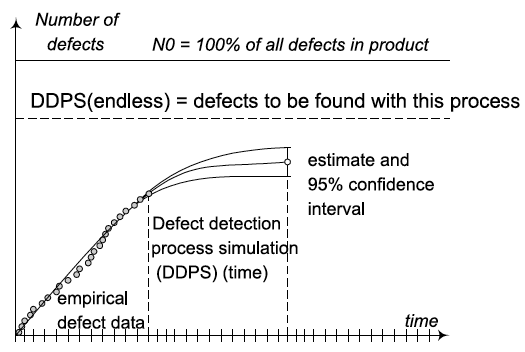
\includegraphics[width=0.7\textwidth]{images/3_2_1.png}
	\caption{Jelinski-Moranda Modell}
	\label{fig:3_2_1_png}
\end{figure}

Hier wird das Jelinksi-Moranda Model vorgestellt. Es zeigt auf, dass mit längerer vergangener Zeit mehr Fehler gefunden werden. Dieses Modell zeigt auf, wieviele Fehler man mit einem bestimmten eingesetzten Modell voraussichtlich finden wird. Eine sehr wichtige Komponente in diesem Modell behandelt das Speichern der Anzahl der Fehler pro Inspektor und in welcher Zeit. Mit diesen Werten ist es möglich das bestehende Modell zu erweitern. Dadurch ergibt sich die Möglichkeit festzustellen wie groß das Fehlerfindungsspektrum eines Inspektors ist. Wenn es zu mehreren Überlappungen der gefundenen Fehler pro Inspektor kommt, dann wird es nur möglich sein einen zentralen Fehleranteil festzustellen. Wenn wir aber zusätzlich Inspektoren einsetzen die auch etwas außerhalb des Zentrums Fehler finden, dann können wir dafür sorgen, dass die Fehlerfindungsrate gesteigert werden kann. Durch die Erstellung von Teams bestehend aus zentralen Inspektoren und Inspektoren die mehr Fehler in den Details finden erhöht man die Fehlerfindungsrate immens.

\begin{figure}
	\centering
	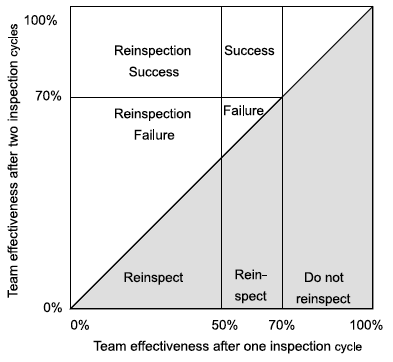
\includegraphics[width=0.7\textwidth]{images/3_2_2.png}
	\caption{Beurteilung 1.Analysezyklus}
	\label{fig:3_2_2_png}
\end{figure}

Um nun den ersten Analysezyklus beurteilen zu können, stellen wir folgenden Schlüssel auf. Wir müssen eine Neuinspektion durchführen, wenn die Fehlerfindungsrate nach dem 1.Zyklus unter 70\% ist und die Chance mit einem 2.Zyklus die 70\% zu übersteigen gegeben ist. Die zweite Möglichkeit wäre die Teams die über 50\% erreicht haben mit Teams die unter 50\% erreicht haben zu vermischen um dadurch eine höhere Fehlerfindungsrate zu erzeugen.
\\ \\
Nachdem wir ein akzeptables Ergebnis mit dieser Wachstumsmethode erreichen konnten, zeigen wir mit zwei heuristischen linearen Modellen, dass dieses Ergebnis unterstrichen werden kann. Wer kombinieren ein optimistisches Modell und ein pessimistisches Modell um die Fehlerfindungsrate über 70\% bringen zu können. 
\\ \\
Hierzu wurde ein Experiment an über 200 Studenten durchgeführt die ein mittelgroßes Projekt planen sollten. Die Studenten hatten jedoch kein gleich hohes Level über die Entwicklung von Projekten, sondern waren vom Standpunkt her durchgemischt. Die Studenten sollten alle möglichen Fehler finden, die im Projekt auftreten könnten.

\begin{figure}
	\centering
	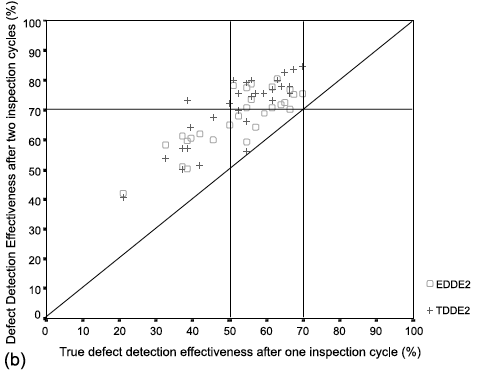
\includegraphics[width=0.7\textwidth]{images/3_2_3.png}
	\caption{Einordnung der gefundenen Fehler}
	\label{fig:3_2_3_png}
\end{figure}

Zur Analyse wurden 29 Teams von Inspektoren eingesetzt zur Aufdeckung der Fehler. Nach einem 1.Analysezyklus konnten 52,5\% (Abweichung von 12,2\%) aller Fehler entdeckt werden. Nach einem 2.Analysezyklus konnten 70,1\% (Abweichung von 11,6\%) aller Fehler entdeckt werden. Durch Gegenüberstellung der Ergebnisse aus dem 1.Zyklus mit den Ergebnissen aus dem 2.Zyklus und der Darstellung in den oben gezeigten Wachstumsmodell, orientieren sich die Ergebnisse großteils im Erfolgsbereich.
\\ \\
Damit man nun die Effektivität besser aufzeigen kann, erstellen wir drei lineare Modelle aus unserem Wachstumsmodell, sowie aus den Beziehungen der Ergebnisse vom 1.Zyklus mit dem 2.Zyklus bezüglich der Effektivität und der Anzahl gefundener Fehler und abstrahieren das in ein Modell, welches die Fehlerfindungsrate nach zwei Zyklen mit der maximalen Anzahl an Fehlern gegenüberstellt und erkennen, dass die Fehlerfindungsrate nach zwei Zyklen sich sich zu einem großen Prozentsatz in einem Bereich zwischen 65 und 80 Prozent befinden. Mit diesen Ergebnissen im Hintergrund kann ein Projektmanager ohne zu zögern in die nächste Phase eintauchen.


\subsection{Integrating Collaborative Processes}

\subsection{A Family of Experiments to investigate the effects of groupware}

Aufgrund der Vorartikel ist bekannt, dass Softwareinspektion eine Angelegenheit ist die sehr viel Ressourcen und Planung benötigt um die Qualität des zu entstehenden Produkts auf ein zielgerichtetes Maß zu bringen. Viele Bereiche der Softwareinspektion können automatisch ohne einen Menschen durchgeführt werden. In diesem Sinne ist es sinnvoll seine Fähigkeiten in die Bereiche einzubringen in denen man den Mensch benötigt und den anderen Teil von einer Software erledigen zu lassen. In dem Artikel “A Family of Experiments to investigate the effects of groupware” von Stefan Biffl wird der Gruppen unterstützte Inspektionsprozess (GRIP) erklärt und mittels Experimenten unter Studenten getestet, wie sinnvoll der Einsatz solcher Tools im Softwareinspektionsbereich ist. Das Ergebnis dieser Experimente hat gezeigt, dass sich Inspektoren viel weniger oft treffen müssen und trotzdem gute Ergebnisse erzielen. Außerdem können falsch positive Fehler schneller aufgedeckt werden und die Anzahl der richtigen Fehler die innerhalb eines Meetings vergessen wurde, wird verringert, jedoch konnte man nicht die Rate der falsch positiven senken. Dieser Wert ist konstant gleich hoch geblieben.
\\ \\
Der Aufbau eines Inspektionsprozesses besteht aus zwei wichtigen Komponenten. Die erste Komponente befasst sich mit der Fehlerfindung. In dieser Komponente sind die einzelnen Inspektoren auf sich alleine gestellt und versuchen so viele Fehler als möglich zu identifizieren. Die zweite Komponente ist das Inspektionsmeeting. In diesem Meeting treffen alle Inspektoren zusammen um ihre Ergebnisse auf den Tisch zu legen und darüber zu diskutieren. Es wurde jedoch mit Experimenten bewiesen, dass die zweite Komponente sehr kostspielig ist und der Erfolg nicht dem entspricht was man sich wünschen würde.
\\ \\
In dem Artikel von Stefan Biffl geht es darum einen Gruppen unterstützten Inspektionsprozess zu implementieren, der die beiden Komponenten effizienter machen soll, sowie die Vorteile der Komponenten zu stärken und Schwächen zu mildern. Zu diesem Zweck wurde ein Prozess erstellt der es ermöglichen sollte Gruppen von Inspektoren effizienter in deren Arbeit zu machen.
\\ \\
Motivation für die Findung eines besseren Prozesses als die Bestehenden war die, dass viele computergestützte Tools nur für die Programmcode Inspektion gedacht sind. Außerdem haben verschiedenste Tools immer nur einen Inspektionsprozess implementiert, sodass sich die Anzahl der möglichen Einsatztools schnell verringert hat.

\begin{figure}
	\centering
	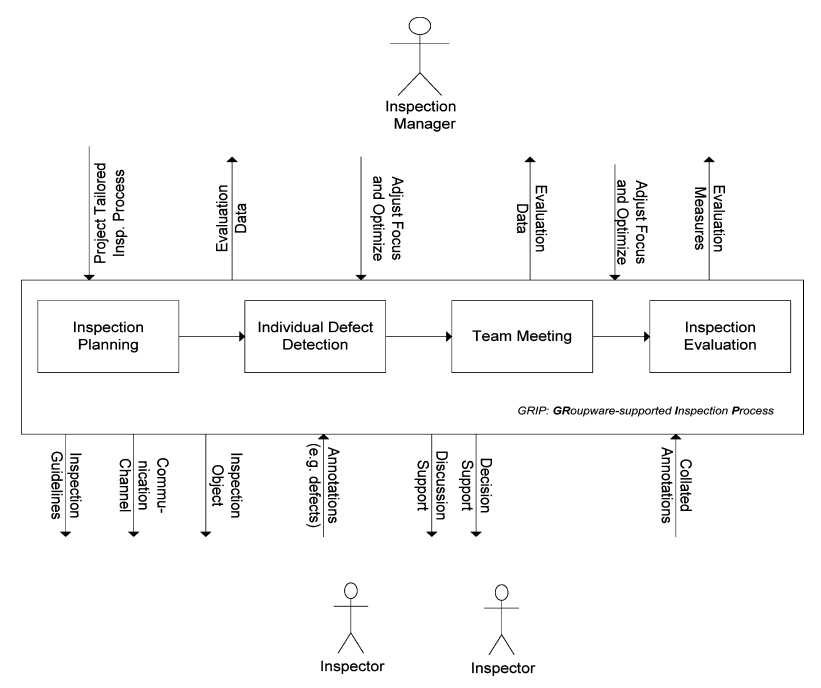
\includegraphics[width=0.7\textwidth]{images/3_4_1.png}
	\caption{Einordnung der gefundenen Fehler}
	\label{fig:3_4_1_png}
\end{figure}

Der Gruppen unterstützte Inspektionsprozess von Stefan Biffl inkludiert die Wünsche der Nutzer. Der Prozess beinhaltet eine Planungsphase, verschiedenste Fehlererkunngsmöglichkeiten, unterstützt Inspektionsmeetings, eine Möglichkeit zum Vergleichen von Fehlern und eine Analysemöglichkeit über die Inspektionseffizienz. Damit dieser Prozess funktionieren kann müssen zwei Rollen erläutert werden. Zum einen gibt es einen Inspektionsmanager der den Inspektionsprozess plant und überwacht. Der Inspektionsmanager überwacht sämtliche Meetings und Abläufe der Inspektoren und verbessert - wenn nötig - die einzelnen Bereiche. Die zweite wichtige Rolle beinhaltet den Inspekteur. Dieser muss seine gefundenen Fehler elektronisch vermerken und bekommt automatisiert eine Übersicht über Überschneidungen von Fehlern, sowie eine Möglichkeit in alle Fehler einzublicken.
\\ \\
Diese Aufteilung und die Benützung von computergestützten Tools ermöglicht es einen höheren Informationsaustausch zu garantieren. Außerdem schafft man damit eine Möglichkeit sich Einblick in alle gemeldeten Fehler zu verschaffen, was vorher nur über Meetings vereinfacht möglich war. Durch die Virtualisierung von Dokumenten schafft man die Möglichkeit mehrere Dokumente gleichzeitig nach Stichworten zu durchsuchen um effizienteres Suchen zu ermöglichen.
\\ \\
Stefan Biffl versucht in seinem Artikel mittels Experimenten herauszufinden, ob diese Vorteile auch wirklich zutreffen oder ob das Arbeiten am Papier noch lange nicht ausgestorben ist. Hierzu werden vier Testkriterien herangezogen. 
Bei der Effektivität der Fehlerfindung geht es darum herauszufinden ob die Findung von doppelten Fehlern minimiert werden kann über allen Inspektoren. Die Effizienz der einzelnen Inspektoren soll untersucht werden. Außerdem soll festgestellt werden ob die Arbeitszeit der Inspektoren minimiert wird. 
\\ \\
Insgesamt wurden drei Experimente durchgeführt, wobei zwei davon mit Papier und Stift, aber unterschiedlichen Lesemethoden, durchgeführt wurden und ein Experiment mit dem neuen Gruppen unterstützten Inspektionsprozess. Das letzte Experiment benutzt die gleiche Lesemethode wie eines der beiden anderen Experimente um später einen besseren Vergleich erreichen zu können. 
\\ \\
Die Ergebnisse des Experiments waren einerseits verblüffend und andererseits bestätigend. Zum Beispiel konnte gezeigt werden, dass die Aufdeckungsrate aller Fehler im Projekt, welche mit dem GRIP Prozess gefunden wurden, um einige Prozent schlecht war als die Aufdeckungsrate mit der Papier und Stift Methode, jedoch nicht signifikant unterschiedlich. 
\\ \\
Ein Vorteil des GRIP Prozesses gegenüber den bestehenden Methoden liegt darin, dass dieser weniger Zeit in Anspruch nimmt. Es konnte gezeigt werden, dass aufgrund des einfachen Informationaustausches es möglich war die durchschnittliche Arbeitszeit der Inspektoren zu verringern, weil sie Einsicht in alle gemeldeten Fehler hatten und somit schneller einen Überblick gewinnen konnten. Dies führt automatisch dazu, dass die Anzahl der doppelt gemeldeten Fehler signifikant verringert werden konnte. Im Vergleich zu den Papier Experimenten konnte man um die Hälfte weniger Mehrfachmeldungen vermerken. 
\\ \\
Eine wesentliche Komponente des Inspektionsprozesses sind die Team Meetings. Wie wir am Anfang festgestellt hatten, verliert man im Team Meeting schnell den Überblick und meldet schnell falsche Fehler als richtige. Im GRIP Prozess konnte gezeigt werden, dass die Computerunterstützung dabei helfen konnte, weniger Fehler zu vergessen bzw. zu verlieren. Aufgrunddessen wurden auch weniger falsche Fehler als positive vermerkt. Dies bedeutet, dass die Effizienz der Gruppenmeetings deutlich gesteigert werden konnte und die Fehlerraten verbessert werden konnten. 
\\ \\
Zusammenfassend stellt man fest, dass einige Methodiken auf dem Papier sinnvoller sind als mit einem Tool, jedoch wenn man die Gesamtheit betrachtet es zu vielen Vorteilen kommt, wenn man den Inspektionsprozess mithilfe des richtigen Tools plant und durchführt. Durch den Einsatz von GRIP konnte man zeigen, dass Kosten eingespart werden können und Ressourcen erzeugt werden können. Die exzellente Planbarkeit, sowie Verfolgbarkeit jedes einzelnen Schritts im Tool ermöglicht eine genaue Analyse und eine effizientere Abarbeitung der einzelnen Schritte und Prozesse in der Inspektion.

\section{Zusammenfassung}

% VORLAGEN FÜR DINGE 
% #####################################################################################

\section{Vorlagen}

\subsection{Tables}
Tables have to be realized with the help of the \textit{table} environment. Tables shall be sequentially numbered for each chapter and described in terms of a short caption (cf. Table~\ref{tab:diplomaseminar}).

\begin{table}[htb]
	\centering
	\begin{tabular}{|l|c|c|}
		\hline \textbf{Name} & \textbf{Date} & \textbf{Title} \\
		\hline
		\hline Mustermann Adam  & 18.5   & T1    \\
		\hline Musterfrau Eva  & 22.6   & T2    \\
		\hline
	\end{tabular}
	\caption{Seminar for Master Students}
	\label{tab:diplomaseminar}
\end{table}


\subsection{Figures}

Like tables, figures shall be sequentially numbered for each chapter and described in terms of a short caption). You could either produce your drawings directly inside Latex using PSTricks\footnote{\url{http://tug.org/PSTricks}}, Tikz\footnote{\url{http://sourceforge.net/projects/pgf}}, or any set of macros dedicated to your requirements (cf. Figure~\ref{fig:samplefigure_tikz}). Alternatively, you may include figures prepared in external tools (cf. Figure~\ref{fig:samplefigure_pdf}). Note, to ensure high quality printing, all figures must have at least 300 dpi.

\begin{figure}
	\centering
	\begin{tikzpicture}[->, auto, node distance=2.8cm, semithick]
	  \node[initial, state] (1)		 {$S_1$};
	  \node[state] 		(2) [right of=1] {$S_2$};
	
	  \path (1) edge [bend left]  node {0} (2)
		(1) edge [loop above] node {1} (1)
		(2) edge [bend left]  node {0} (1)
		(2) edge [loop above] node {1} (2);
	\end{tikzpicture}
	\caption{Sample figure}
	\label{fig:samplefigure_tikz}
\end{figure}

\begin{figure}[tb]
	\centering
	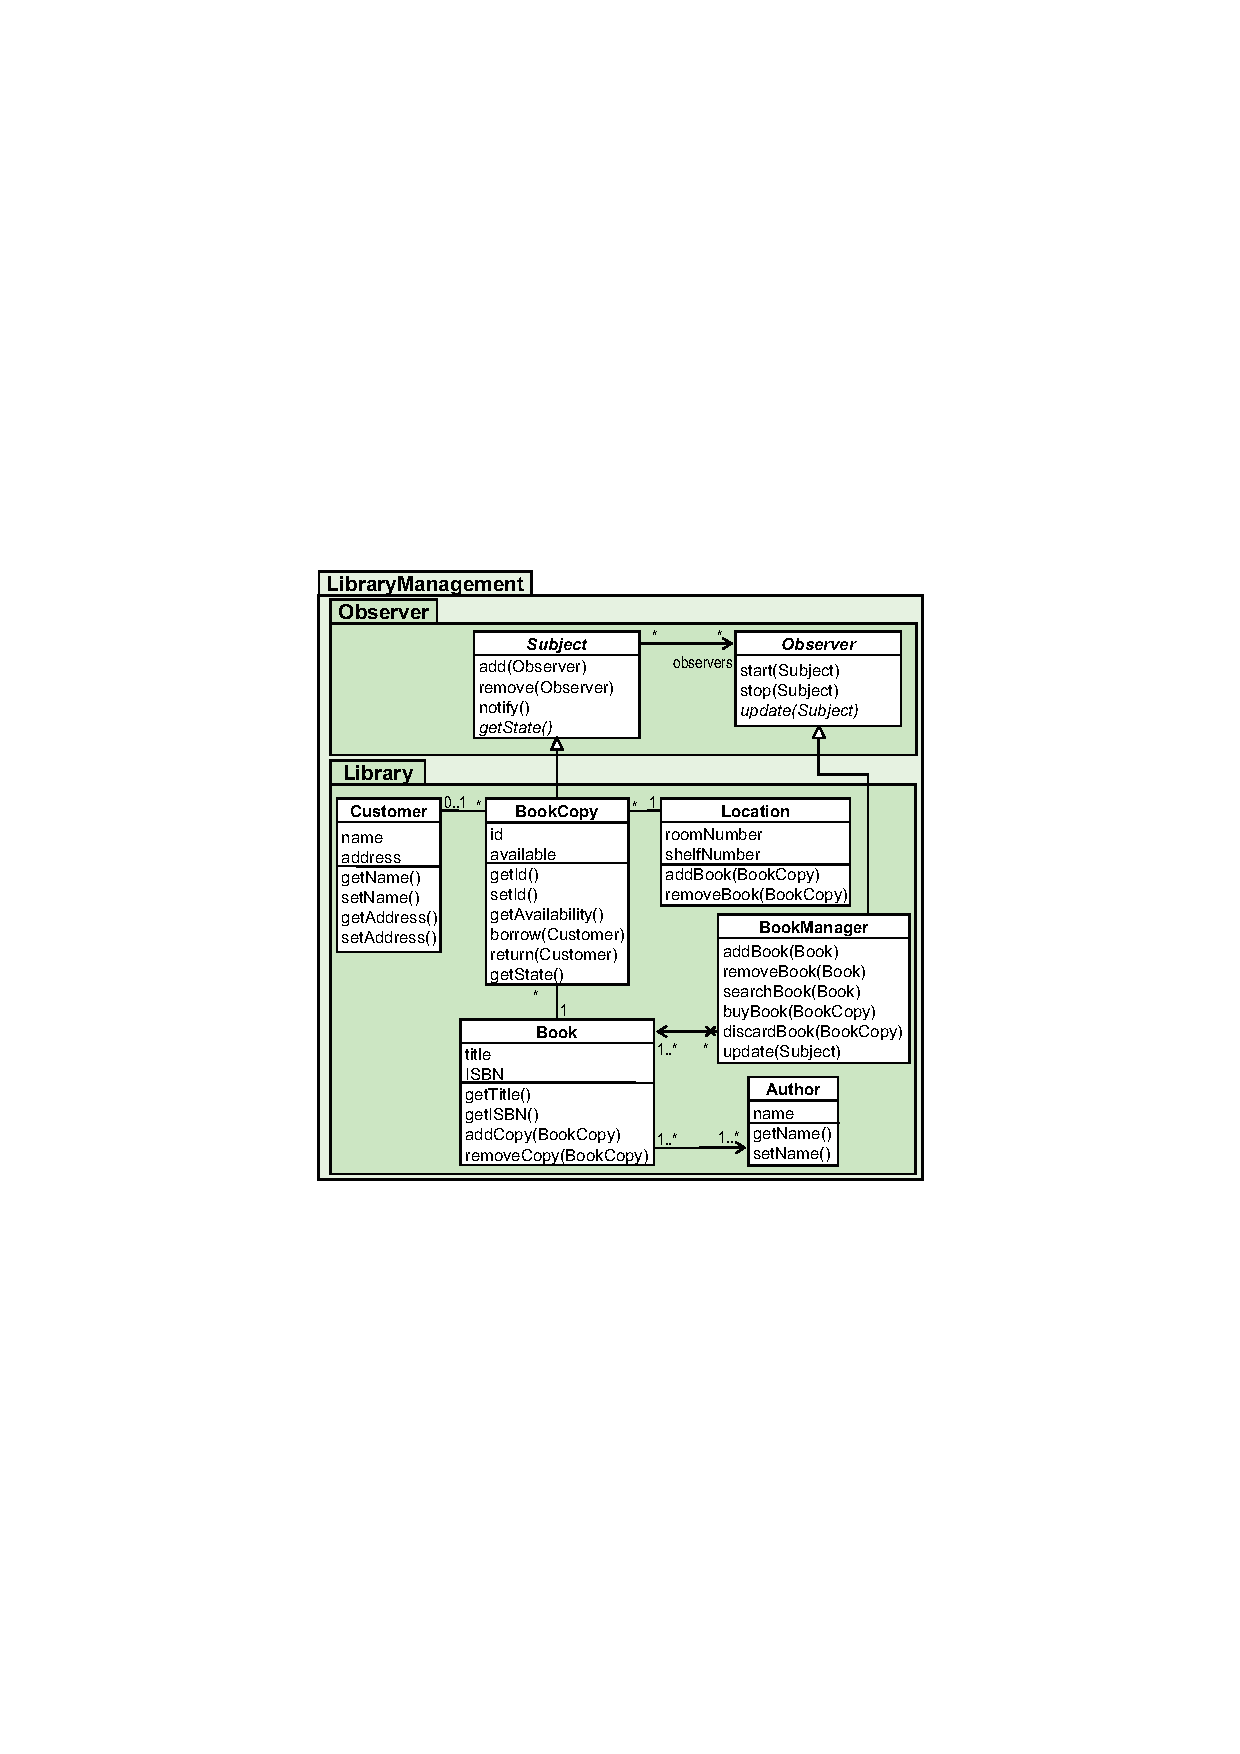
\includegraphics[width=0.7\textwidth]{figures/figure1}
	\caption{Sample figure}
	\label{fig:samplefigure_pdf}
\end{figure}


\subsection{Fonts}

When introducing important terms for the first time use \emph{emphasize}. For a consistent look and feel of proper names like {\cd} and {\uml{Observer}} pattern you may define macros in the main document \texttt{thesis.tex}.

\subsection{Code}

For short code fragments use the \textit{verbatim} environment.

\begin{verbatim}
//Start Program
System.out.println("Hello World!");
//End Program
\end{verbatim}

A much better alternative is the \textit{algorithm} environment (cf. Algorithm~\ref{alg:samplealgorithm}). This environment offers special formatting features for loops, operations and comments.

\begin{algorithm}[t]
\SetKwData{Left}{left}
\SetKwData{This}{this}
\SetKwData{Up}{up}
\SetKwFunction{Union}{Union}
\SetKwFunction{FindCompress}{FindCompress}
\SetKwInOut{Input}{input}
\SetKwInOut{Output}{output}

\Input{A bitmap $Im$ of size $w\times l$}
\Output{A partition of the bitmap}

\BlankLine

\emph{special treatment of the first line}\;
\For{$i\leftarrow 2$ \KwTo $l$}{
\emph{special treatment of the first element of line $i$}\;
\For{$j\leftarrow 2$ \KwTo $w$}{\label{forins}
\Left$\leftarrow$ \FindCompress{$Im[i,j-1]$}\;
\Up$\leftarrow$ \FindCompress{$Im[i-1,]$}\;
\This$\leftarrow$ \FindCompress{$Im[i,j]$}\;
\If(\tcp*[r]{O(\Left,\This)==1}){\Left compatible with \This}{\label{lt}
\lIf{\Left $<$ \This}{\Union{\Left,\This}}\;
\lElse{\Union{\This,\Left}\;}
}
\If(\tcp*[r]{O(\Up,\This)==1}){\Up compatible with \This}{\label{ut}
\lIf{\Up $<$ \This}{\Union{\Up,\This}}\;
\tcp{\This is put under \Up to keep tree as flat as possible}\label{cmt}
\lElse{\Union{\This,\Up}}\tcp*[r]{\This linked to \Up}\label{lelse}
}
}
\lForEach{element $e$ of the line $i$}{\FindCompress{p}}
}
\caption{Sample algorithm}\label{alg:samplealgorithm}
\end{algorithm}

\section{Bibliographic Issues}

\subsection{Literature Search}

Information on online libraries and literature search, e.g., interesting magazines, journals, conferences, and organizations may be found at \url{http://www.big.tuwien.ac.at/teaching/info.html}.

\subsection{BibTeX}

BibTeX should be used for referencing.

The LaTeX source document of this pdf document provides you with different samples for references to journals~\cite{jour:B2BServices}, conference papers~\cite{proc:TheWebMLApproach}, books~\cite{book:umlatwork}, book chapters~\cite{incoll:ErhardKonrad1992}, electronic standards~\cite{man:BPEL}, dissertations~\cite{phdthesis:manuelWimmer}, masters' theses~\cite{mast:AUMLProfile}, and web sites~\cite{misc:BIGWebsite}. The respective BibTeX entries may be found in the file \texttt{references.bib}. For administration of the BibTeX references we recommend \url{http://www.citeulike.org} or JabRef for offline administration, respectively.

\bibliographystyle{acm}
\bibliography{references}

\end{document}
